\documentclass[12pt, a4paper]{article}

% ===== 中文支持 =====
\usepackage[UTF8, zihao=-4]{ctex}

% ===== 页边距 =====
\usepackage[top=2.5cm, bottom=2.5cm, left=2.8cm, right=2.8cm]{geometry}

% ===== 字体 =====
\usepackage{fontspec}
\setmainfont{Times New Roman}

% ===== 行距 =====
\usepackage{setspace}
\setstretch{1.5}
\setlength{\parskip}{0pt}

% ===== 插图 =====
\usepackage{graphicx}
\usepackage{float}
\graphicspath{{./实验照片/}{./media/}}

% ===== 表格 =====
\usepackage{booktabs}
\usepackage{array}
\usepackage{multirow}

% ===== 数学公式 =====
\usepackage{amsmath, amssymb}

% ===== 图表编号（章-序号格式） =====
\usepackage{chngcntr}
\renewcommand{\thefigure}{\arabic{section}-\arabic{figure}}
\renewcommand{\thetable}{\arabic{section}-\arabic{table}}
\counterwithin{figure}{section}
\counterwithin{table}{section}

% ===== 图表标题 =====
\usepackage{caption}
\captionsetup{font=small, labelsep=space, justification=centering,
              aboveskip=6pt, belowskip=12pt}
\captionsetup[table]{aboveskip=12pt, belowskip=6pt, position=above}

% ===== 页眉页脚 =====
\usepackage{fancyhdr}
\setlength{\headheight}{15pt}
\pagestyle{fancy}
\fancyhf{}
\fancyhead[C]{\small 杨氏双缝干涉实验\ 实验报告}
\fancyfoot[C]{\small\thepage}

% ===== 目录超链接 =====
\usepackage[colorlinks=true, linkcolor=black, citecolor=black, urlcolor=blue,
            bookmarks=true, bookmarksnumbered=true]{hyperref}

% ===== 章节标题格式（titlesec） =====
\usepackage{titlesec}
\titleformat{\section}[block]
  {\centering\heiti\zihao{4}}{\thesection}{1em}{}
\titlespacing*{\section}{0pt}{24pt}{18pt}
\titleformat{\subsection}[hang]
  {\heiti\zihao{-4}}{\thesubsection}{1em}{}
\titlespacing*{\subsection}{0pt}{18pt}{6pt}

\begin{document}

% ===== 封面 =====
\begin{titlepage}
  \centering
  \vspace*{3cm}
  {\heiti\zihao{2} 实验报告}\\[1cm]
  {\heiti\zihao{3} 杨氏双缝干涉实验}\\[2.5cm]
  \begin{tabular}{ll}
    姓\quad 名： & 叶哲昊 \\[0.6cm]
    学\quad 号： & 24012561 \\[0.6cm]
    班\quad 级： & 24级光电二班 \\[0.6cm]
    实验日期：   & 2026.3.27 \\
  \end{tabular}
  \vfill
\end{titlepage}

\tableofcontents
\newpage
\setcounter{page}{1}

% ===== 第一节：实验目的 =====
\section{实验目的}

\begin{enumerate}
  \item 学习并掌握调节光学系统等高共轴的步骤和方法；
  \item 理解杨氏双缝干涉现象的基本原理；
  \item 掌握杨氏双缝干涉实验光路及其调整方法；
  \item 观察杨氏双缝干涉现象，并掌握一种利用干涉条纹间距测量光波波长的方法。
\end{enumerate}

% ===== 第二节：实验原理 =====
\section{实验原理}

杨氏双缝干涉利用分波面法获得相干光。激光经空间滤波器和准直透镜后形成近似平行光，
照射双缝后在缝后方$D$处的接收屏上产生等间距干涉条纹，实验原理如图~\ref{fig:principle}~所示。

\begin{figure}[H]
  \centering
  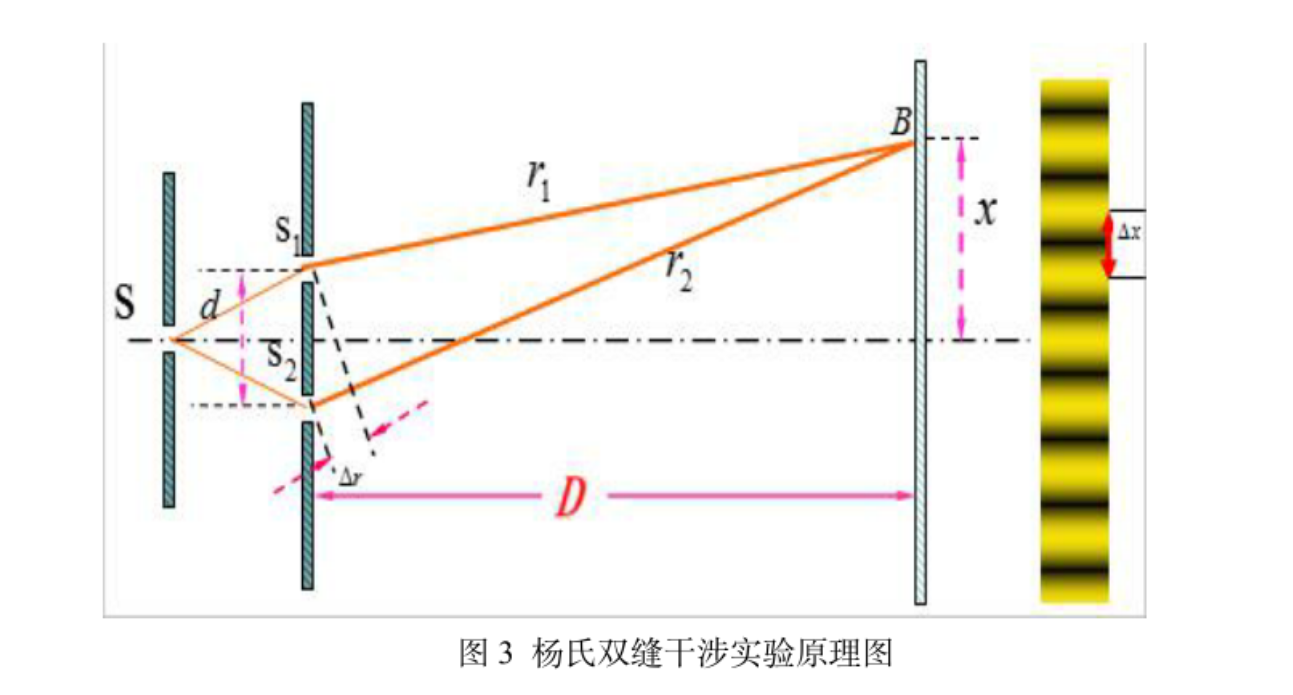
\includegraphics[width=0.70\textwidth]{3.png}
  \caption{杨氏双缝干涉实验原理图}
  \label{fig:principle}
\end{figure}

设两缝$S_1$、$S_2$的缝间距为$d$，双缝到接收屏的垂直距离为$D$，屏上任意一点$P$的坐标为$x$，
$S_1$、$S_2$到$P$点的距离分别为$r_1$和$r_2$，由几何关系得：
\begin{equation}
  r_1^2 = D^2 + \left(x - \frac{d}{2}\right)^2, \quad
  r_2^2 = D^2 + \left(x + \frac{d}{2}\right)^2
\end{equation}

两式相减并利用$D \gg d$、$D \gg x$，得$r_1 + r_2 \approx 2D$，从而光程差为：
\begin{equation}
  \Delta = r_2 - r_1 = \frac{dx}{D}
\end{equation}

\subsection{干涉条件}

明纹（相长干涉）：$\Delta = k\lambda$（$k = 0,\pm1,\pm2,\cdots$）；
暗纹（相消干涉）：$\Delta = (2k+1)\dfrac{\lambda}{2}$（$k = 0,\pm1,\pm2,\cdots$）。

\subsection{条纹间距与波长公式}

相邻明纹（或暗纹）间距相等，记为$\Delta x$：
\begin{equation}
  \Delta x = \frac{D\lambda}{d}
  \label{eq:fringe_spacing}
\end{equation}

整理得本实验的测量公式：
\begin{equation}
  \lambda = \frac{\Delta x \cdot d}{D}
  \label{eq:wavelength}
\end{equation}

由实验测出$D$、$d$以及$\Delta x$，即可由式~(\ref{eq:wavelength})计算光波波长$\lambda$。

% ===== 第三节：实验仪器 =====
\section{实验仪器}

本实验使用以下光学仪器：
\begin{enumerate}
  \item \textbf{激光器}：输出绿色激光（标称波长约532\,nm），作为单色光源；
  \item \textbf{圆形可调衰减器}：用于调节激光束强度，保护CCD传感器不过曝；
  \item \textbf{空间滤波器}（针孔25\,$\mu$m）：滤除高阶衍射噪声，净化光束；
  \item \textbf{准直透镜}（$\Phi$25.4\,mm，$f$=100\,mm）：将散射球面波变换为平行光束；
  \item \textbf{目标物双缝}（安装于一维平移台）：本次选用B列第4排，
        缝宽$w = 80\,\mu\text{m}$，缝间距$d = 400\,\mu\text{m}$；
  \item \textbf{数字CCD相机}：用于接收并采集干涉条纹图像；
  \item \textbf{监视器}：实时显示CCD图像，供读取条纹位置；
  \item \textbf{一维平移台}（带测微头）：承载CCD，通过读取丝杆读数精确测量条纹间距；
  \item \textbf{米尺}：测量双缝至CCD焦平面的距离$D$；
  \item \textbf{磁性表座及调节支架}：固定和调节各光学元件位置与角度。
\end{enumerate}

实验装置全貌如图~\ref{fig:apparatus}~所示。

\begin{figure}[H]
  \centering
  
\includegraphics[width=0.78\textwidth]{实验装置全貌.jpg}
  \caption{杨氏双缝干涉实验装置全貌}
  \label{fig:apparatus}
\end{figure}

% ===== 第四节：实验步骤 =====
\section{实验步骤}

\subsection{光路搭建与共轴调节}

\begin{enumerate}
  \item \textbf{激光器调平}：借助可变光阑（开孔约2\,mm），在光阑近处和远处分别调节
        激光夹持器的水平俯仰旋钮，反复2次，使出射激光束与光学平台台面平行。

  \item \textbf{调整空间滤波器}：在激光器和光阑之间插入空间滤波器（不加针孔），
        调整位置使物镜出射光斑打在光阑中心；安装针孔（25\,$\mu$m），调节三维旋钮
        使聚焦光斑与针孔重合，观察到圆孔衍射环后再微调至衍射环消失，完成空间滤波。

  \item \textbf{安装准直镜}：在空间滤波器后方安装准直透镜（$f = 100$\,mm），
        调整其高低使出射光束准确入射到光阑中心；前后移动准直镜至远近光斑大小不变，
        表明输出近似平行光束。

  \item \textbf{安装目标双缝}：选择B列第4排双缝（$w = 80\,\mu$m，$d = 400\,\mu$m），
        安装于一维平移台上，置于准直镜后方。观察0级亮斑位置，调整至与光阑中心重合，
        完成共轴调节。

  \item \textbf{安装CCD}：撤去光阑，在较远位置安装数字CCD相机；旋转可调衰减器至
        最暗后接通CCD电源，调节衰减量至监视器画面不过曝，可清晰观察到干涉条纹。
\end{enumerate}

\subsection{数据测量}

\begin{enumerate}
  \item 通过调节CCD下方的平移台，使监视器上的十字线交点位于0级亮纹中央，
        记录此时丝杆读数$X_0$。

  \item 沿同一方向匀速拧动测微头，通过监视器依次寻找连续6条暗纹，
        逐一读取并记录其位置读数$X_0 \sim X_5$（单位：mm）。

  \item 用米尺测量双缝至CCD焦平面的距离$D$，重复测量3次，取平均值$\overline{D}$。
        双缝至屏的距离如图~\ref{fig:distance}~所示。
\end{enumerate}

\begin{figure}[H]
  \centering
  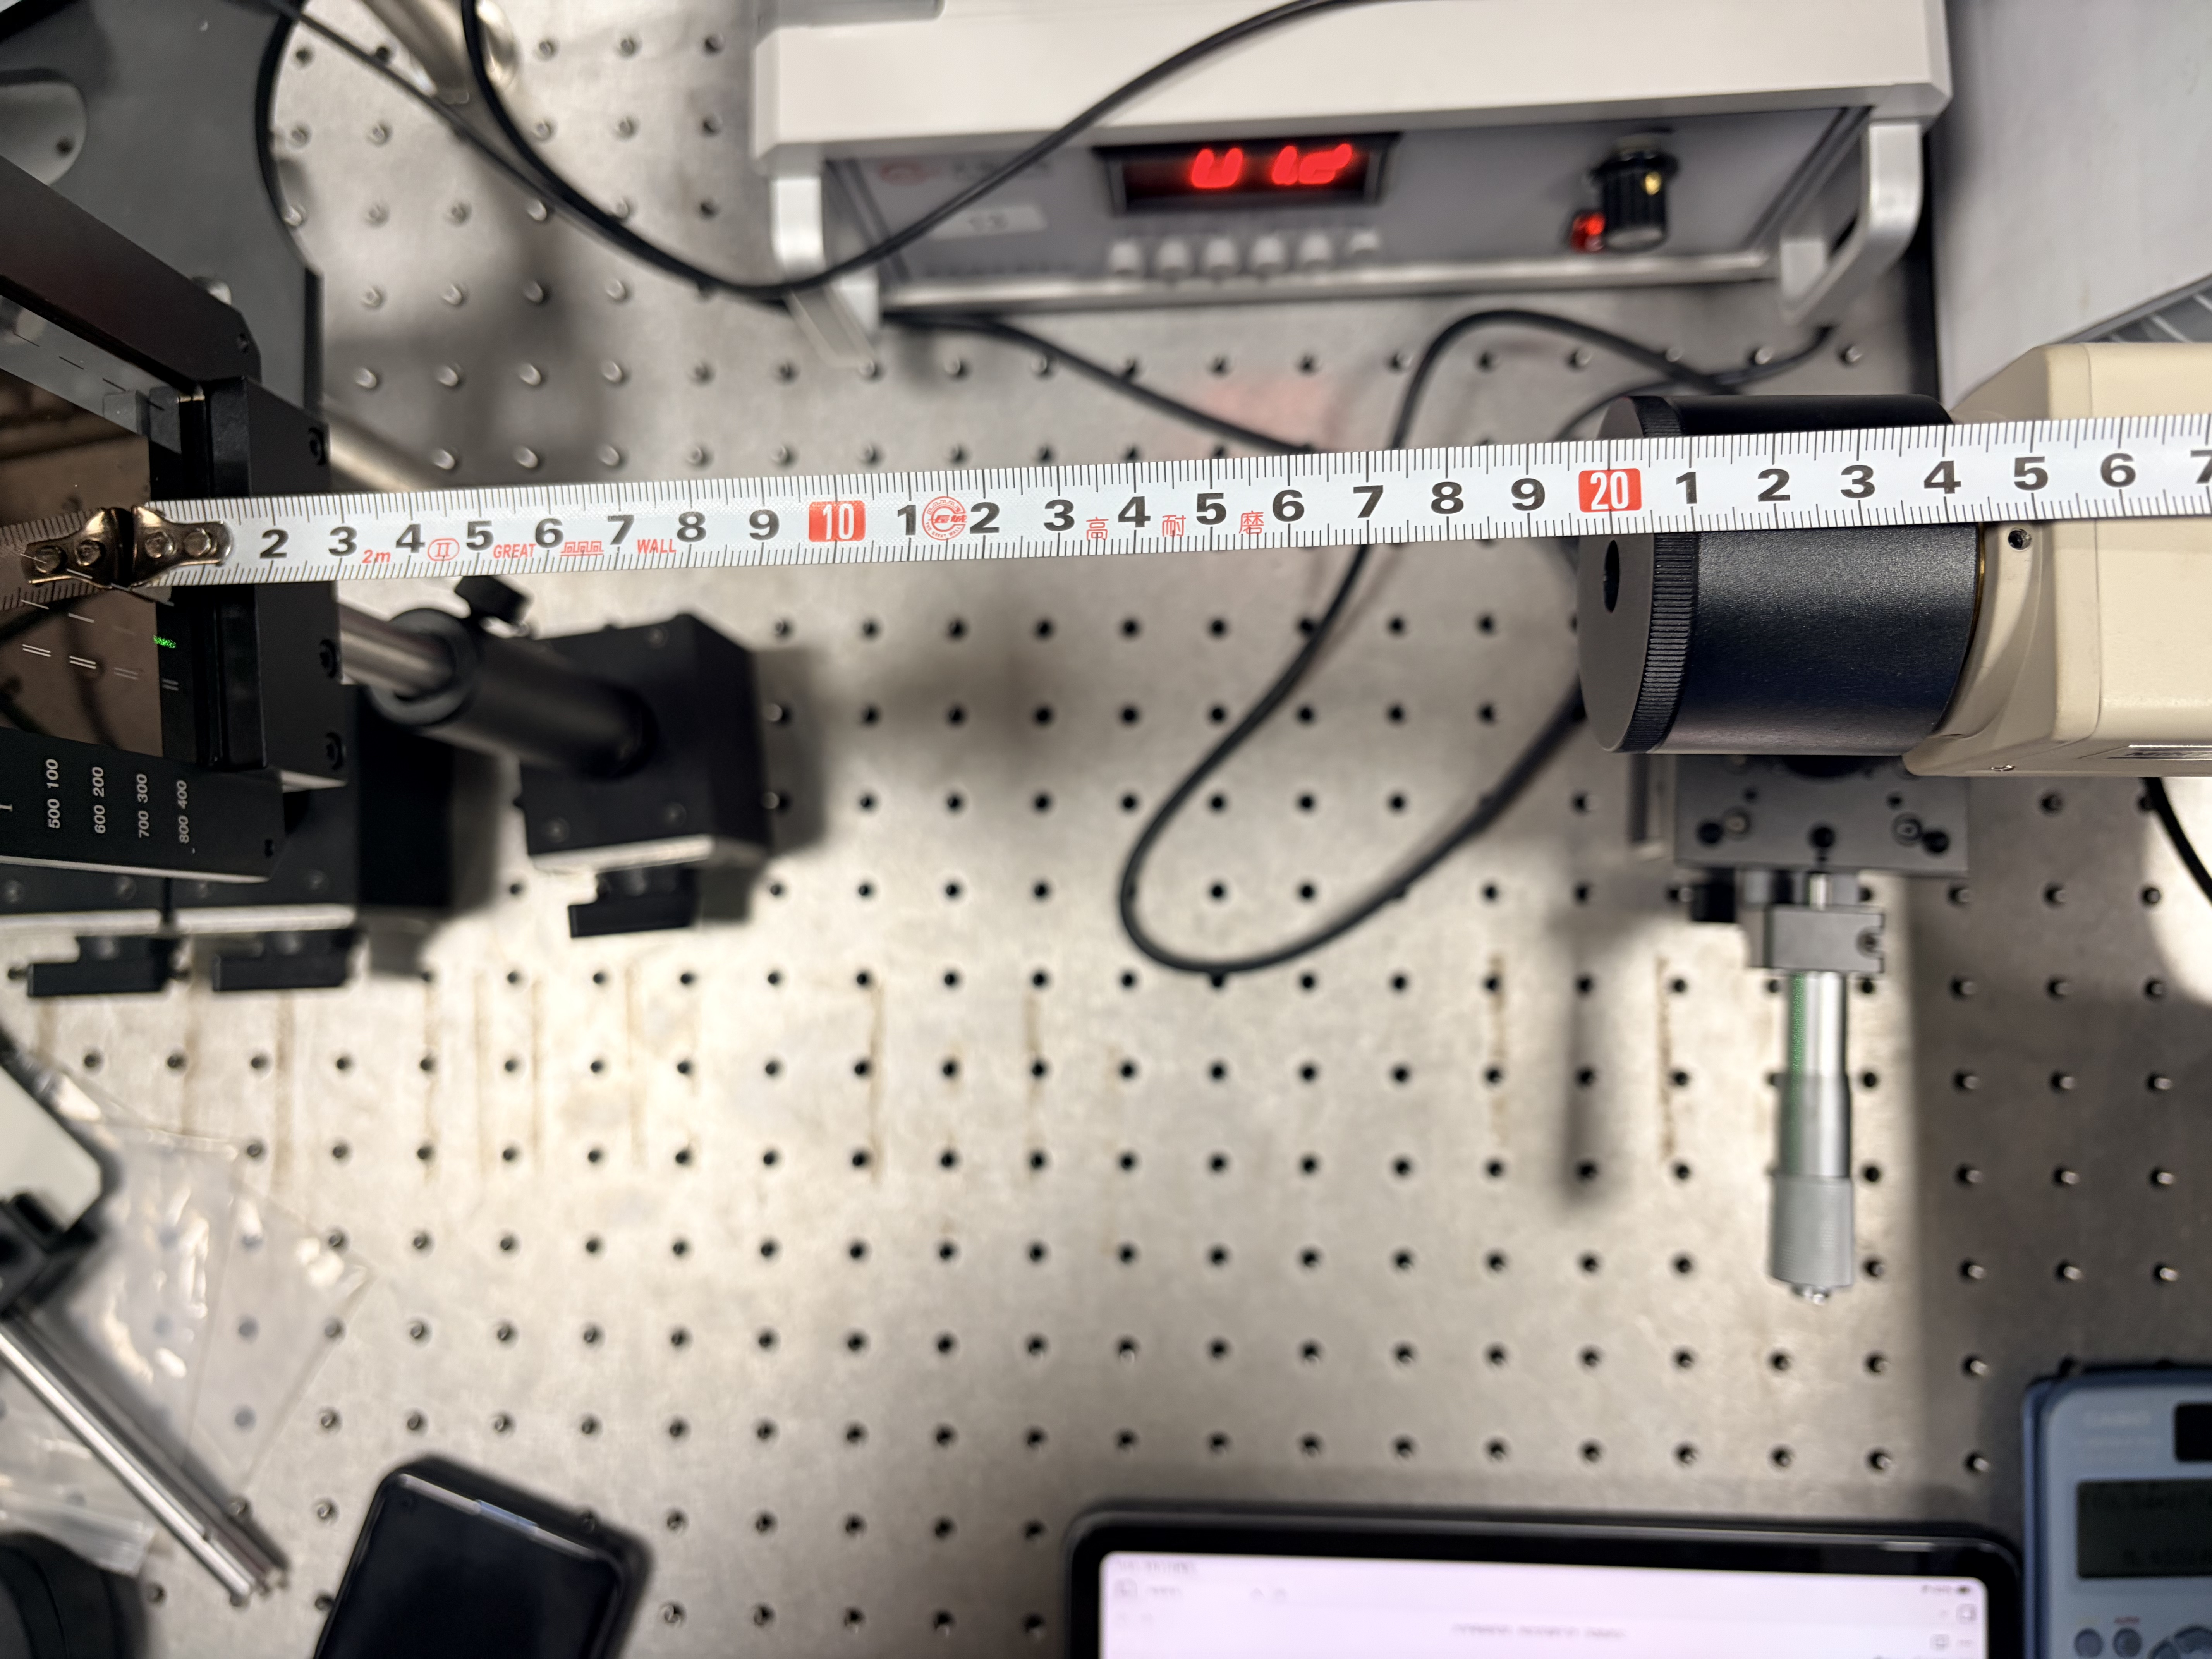
\includegraphics[width=0.72\textwidth]{双缝至屏的25.4cm的间距.jpg}
  \caption{用米尺测量双缝至CCD焦平面距离（$\overline{D} = 25.4$\,cm）}
  \label{fig:distance}
\end{figure}

% ===== 第五节：数据处理（表格部分） =====
\section{实验数据与处理}

\subsection{实验参数记录}

本次实验选用目标物B列第4排双缝，缝宽$w = 80\,\mu\text{m}$，缝间距$d = 400\,\mu\text{m}$。
双缝至CCD焦平面距离$D$的三次测量结果列于表~\ref{tab:D}。

\begin{table}[H]
  \centering
  \caption{双缝宽$w$、缝间距$d$及双缝至屏距离$D$的测量（$w$、$d$单位：$\mu$m；$D$单位：cm）}
  \label{tab:D}
  \begin{tabular}{cccccc}
    \toprule
    $w$/$\mu$m & $d$/$\mu$m & $D_1$/cm & $D_2$/cm & $D_3$/cm & $\overline{D}$/cm \\
    \midrule
    80 & 400 & 25.5 & 25.4 & 25.3 & 25.4 \\
    \bottomrule
  \end{tabular}
\end{table}

\subsection{条纹间距的逐差法测量}

沿同一方向依次读取6条暗纹位置$X_0 \sim X_5$，采用逐差法计算条纹间距$\Delta x$。
设$(\Delta x)_i = \dfrac{X_{i+3} - X_i}{3}$（$i = 0,1,2$），则：
\begin{equation}
  \overline{\Delta x} = \frac{1}{3}\sum_{i=0}^{2}(X_{i+3} - X_i) \cdot \frac{1}{3}
  = \frac{\overline{3\Delta x}}{3}
\end{equation}

测量数据及逐差法结果列于表~\ref{tab:fringe}。
CCD监视器上观察到的干涉条纹如图~\ref{fig:fringes}~所示。

\begin{table}[H]
  \centering
  \caption{逐差法记录条纹间距（单位：mm）}
  \label{tab:fringe}
  \begin{tabular}{ccccc}
    \toprule
    条纹位置（前组） & 数值/mm & 条纹位置（后组） & 数值/mm & $3\Delta x_i$/mm \\
    \midrule
    $X_0$ & 17.160 & $X_3$ & 18.188 & 1.028 \\
    $X_1$ & 17.500 & $X_4$ & 18.520 & 1.020 \\
    $X_2$ & 17.860 & $X_5$ & 18.872 & 1.012 \\
    \midrule
    \multicolumn{4}{c}{$\overline{3\Delta x}$} & 1.020 \\
    \multicolumn{4}{c}{$\overline{\Delta x} = \overline{3\Delta x}/3$} & 0.340 \\
    \bottomrule
  \end{tabular}
\end{table}

\begin{figure}[H]
  \centering
  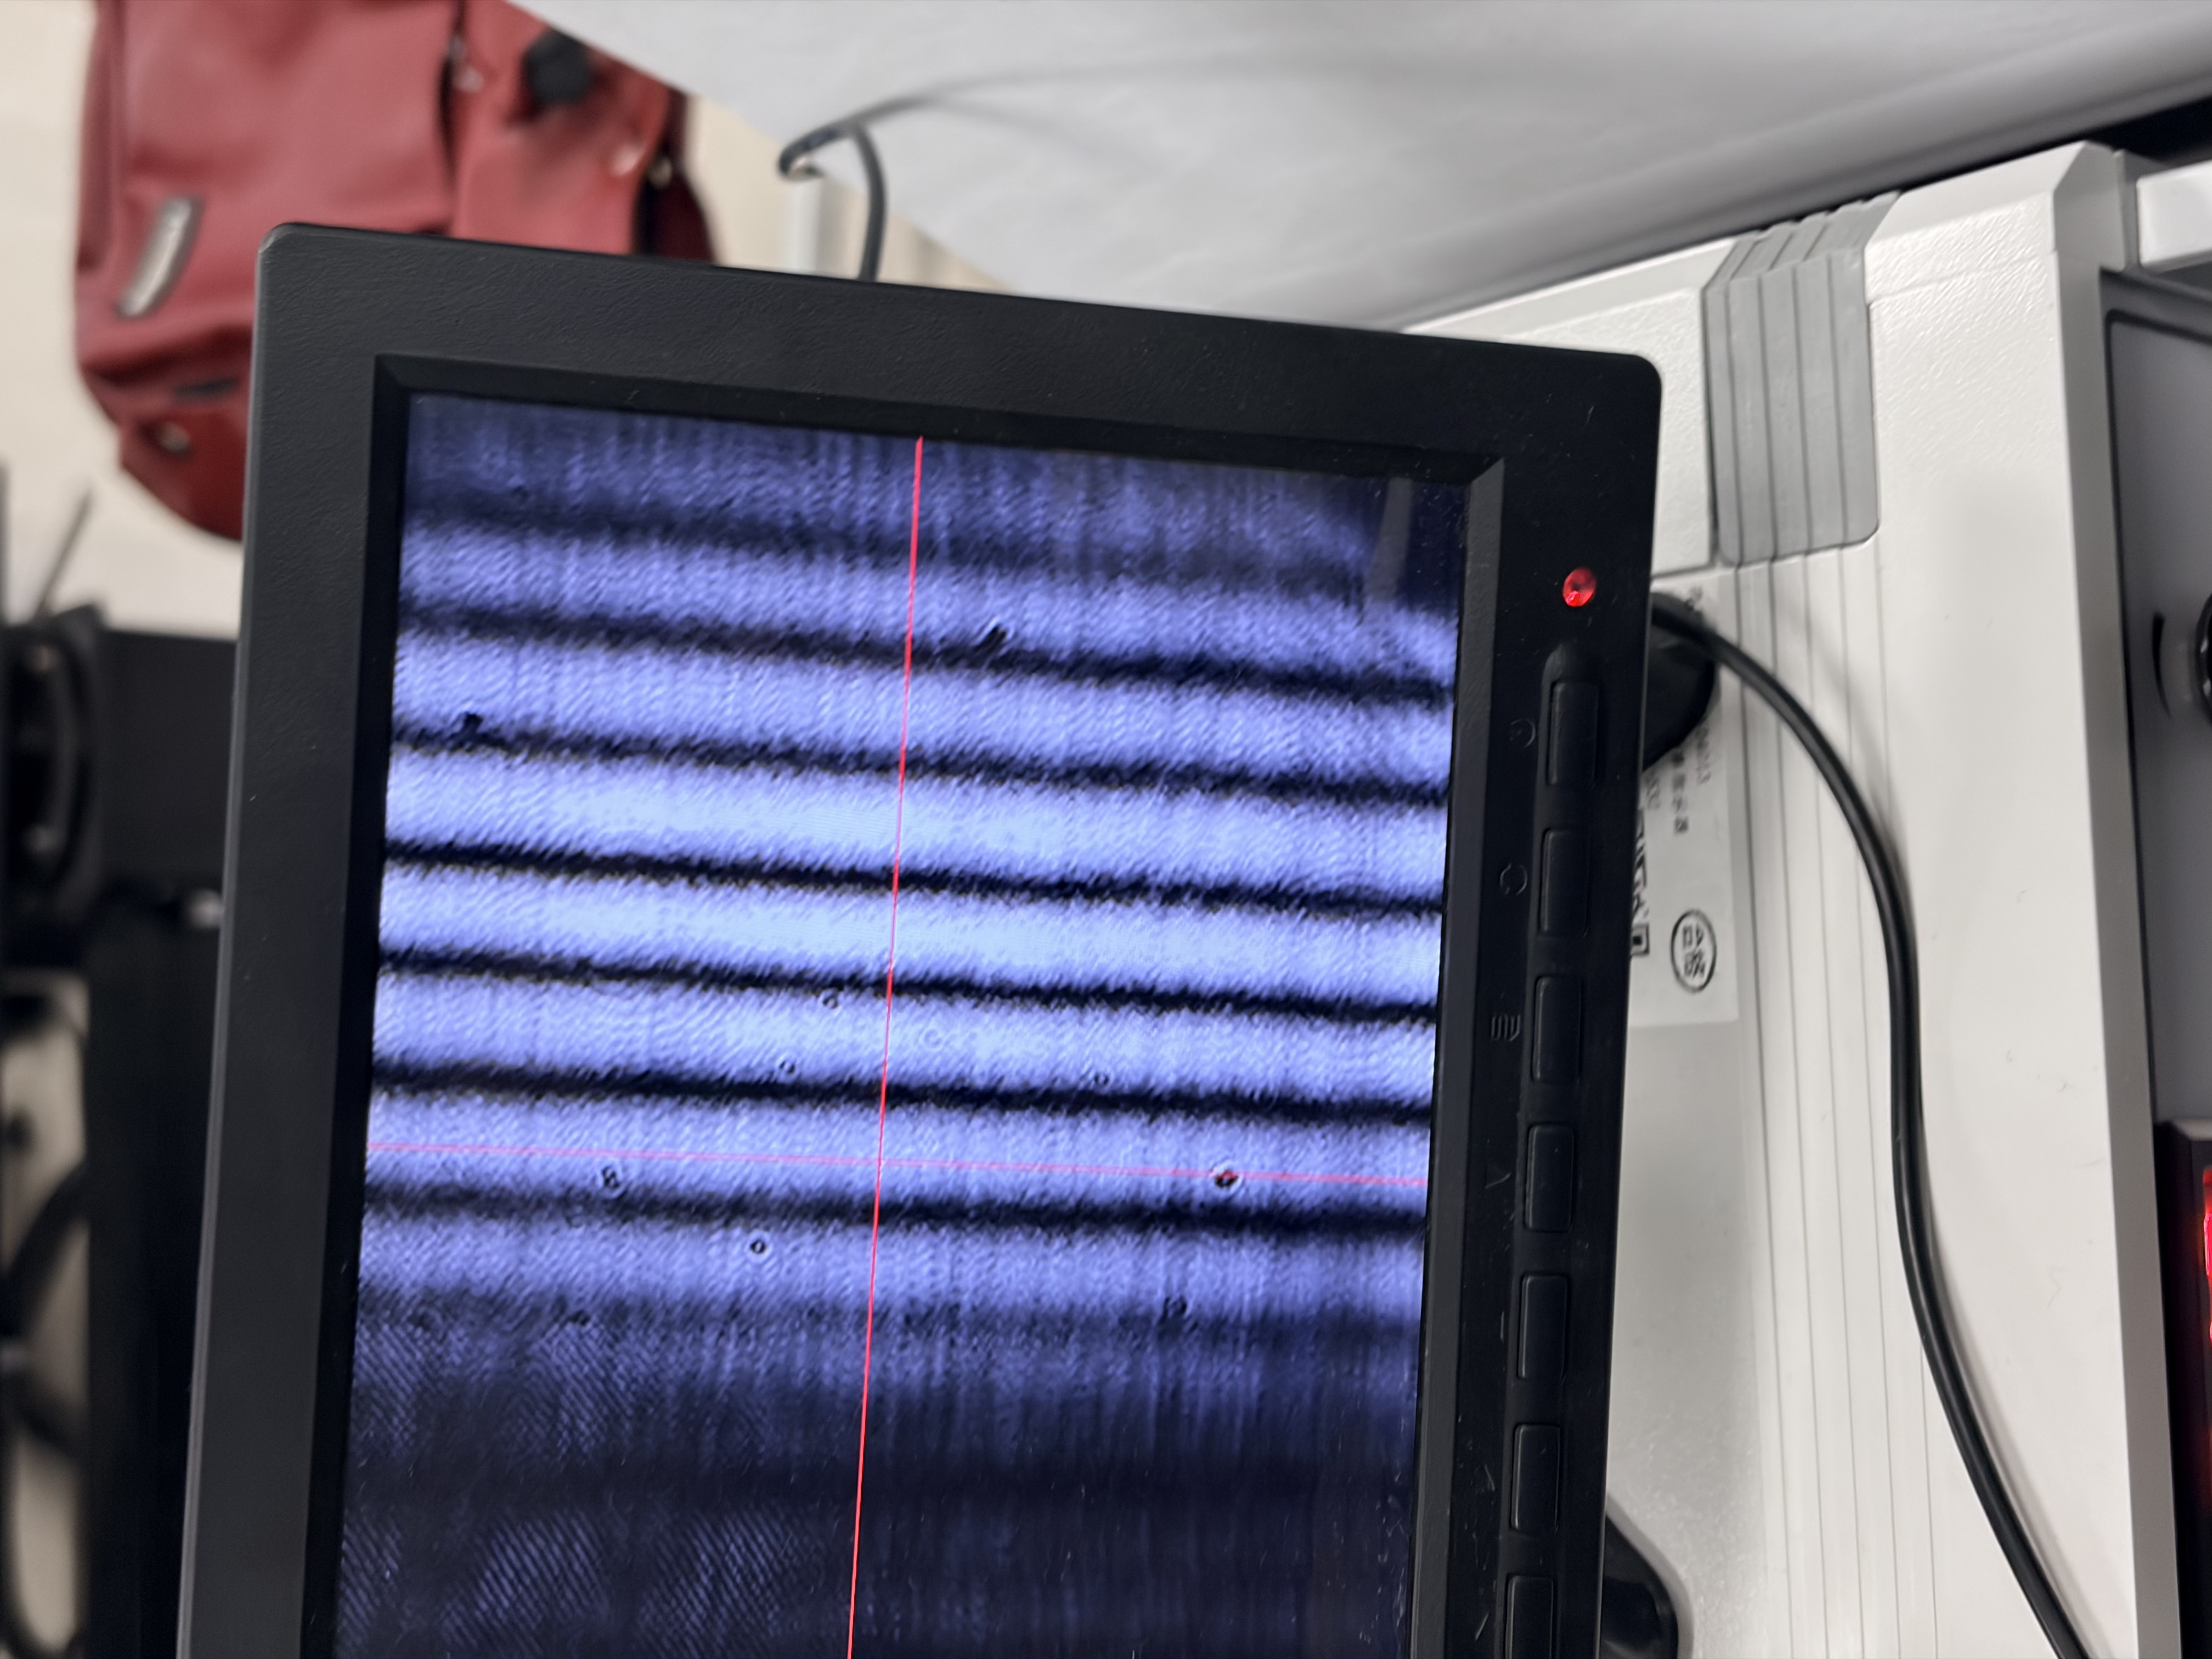
\includegraphics[width=0.62\textwidth]{连接了CCD的显示器上的条纹图样.jpg}
  \caption{CCD监视器上显示的杨氏双缝干涉条纹图样}
  \label{fig:fringes}
\end{figure}

\subsection{波长计算}

将$\overline{\Delta x} = 0.340\ \text{mm}$，$d = 0.400\ \text{mm}$，
$\overline{D} = 254\ \text{mm}$代入式~(\ref{eq:wavelength})：

\begin{equation}
  \bar{\lambda} = \frac{\overline{\Delta x} \cdot d}{\overline{D}}
  = \frac{0.340 \times 0.400}{254}\ \text{mm}
  = 5.354 \times 10^{-4}\ \text{mm}
  \approx 535\ \text{nm}
\end{equation}

\subsection{不确定度评定}

\subsubsection{条纹间距$\overline{\Delta x}$的不确定度}

三组$3\Delta x_i$数据（1.028、1.020、1.012\,mm）的A类不确定度：
\begin{equation}
  s(3\Delta x) = \sqrt{\frac{\sum_{i=0}^{2}(3\Delta x_i - \overline{3\Delta x})^2}{n-1}}
  = \sqrt{\frac{(0.008)^2 + 0 + (-0.008)^2}{2}} = 0.008\ \text{mm}
\end{equation}

\begin{equation}
  u_A(3\Delta x) = \frac{s}{\sqrt{n}} = \frac{0.008}{\sqrt{3}} \approx 0.0046\ \text{mm}
\end{equation}

测微头仪器误差取$\Delta_\text{仪} = 0.001$\,mm，B类不确定度：
$u_B = \Delta_\text{仪}/\sqrt{3} \approx 0.0006$\,mm（可忽略）。

$\overline{\Delta x}$的合成不确定度：
\begin{equation}
  u(\overline{\Delta x}) = \frac{u(3\Delta x)}{3} = \frac{0.0046}{3} \approx 0.0015\ \text{mm}
\end{equation}

\subsubsection{距离$\overline{D}$的不确定度}

三次测量（25.5、25.4、25.3\,cm）的A类不确定度：
\begin{equation}
  s(D) = \sqrt{\frac{(0.1)^2 + 0 + (-0.1)^2}{2}} = 0.100\ \text{cm}, \quad
  u_A(D) = \frac{0.100}{\sqrt{3}} \approx 0.058\ \text{cm}
\end{equation}

米尺最小分度1\,mm，B类不确定度：$u_B(D) = 0.05/\sqrt{3} \approx 0.029$\,cm。
合成不确定度：
\begin{equation}
  u(\overline{D}) = \sqrt{u_A^2 + u_B^2} = \sqrt{0.058^2 + 0.029^2} \approx 0.065\ \text{cm}
\end{equation}

\subsubsection{波长$\lambda$的合成不确定度}

缝间距$d = 400\,\mu$m为标称值，忽略其不确定度。由误差传递公式
$\lambda = \overline{\Delta x} \cdot d / \overline{D}$：
\begin{equation}
  \frac{u(\lambda)}{\bar{\lambda}}
  = \sqrt{\left(\frac{u(\overline{\Delta x})}{\overline{\Delta x}}\right)^2
         + \left(\frac{u(\overline{D})}{\overline{D}}\right)^2}
  = \sqrt{\left(\frac{0.0015}{0.340}\right)^2 + \left(\frac{0.065}{25.4}\right)^2}
  \approx 0.67\%
\end{equation}

\begin{equation}
  u(\lambda) = 0.0067 \times 535 \approx 4\ \text{nm}
\end{equation}

最终测量结果：
\begin{equation}
  \boxed{\lambda = (535 \pm 4)\ \text{nm}}
\end{equation}

与绿色激光标称波长532\,nm相比，相对误差约为0.6\%，结果合理。

% ===== 第六节：误差分析 =====
\section{误差分析}

\begin{enumerate}
  \item \textbf{条纹位置读数误差}：通过监视器目视判断暗纹中心位置时，存在主观判断偏差
        （约$\pm 0.005$\,mm量级），是$\Delta x$不确定度的主要来源。适当增加测量条纹数目
        可有效降低此项误差。

  \item \textbf{距离$D$的测量误差}：米尺测量双缝到CCD焦平面距离时，CCD焦平面的精确位置
        难以直接确定，可能引入约1\,mm的系统偏差。改用更精确的测距工具或多次测量取平均
        可减小此误差。

  \item \textbf{平行光非理想性}：准直后的激光束并非严格平行光，若准直镜位置略有偏差，
        等效光源不在无穷远处，会使条纹间距偏离理论值，引入系统误差。

  \item \textbf{双缝共轴偏差}：若双缝中心未精确位于光轴上，0级条纹可能偏离屏幕中心，
        读数的参考基准发生偏移，但此误差对相邻条纹间距影响较小。

  \item \textbf{缝间距$d$的制造误差}：目标物上标称的缝间距$d = 400\,\mu$m存在一定的
        制造公差（一般在$\pm 2\,\mu$m以内），对最终波长结果引入约0.5\%的系统误差。

  \item \textbf{CCD像素非线性}：CCD在强光区域可能存在饱和或非线性响应，使条纹中心位置
        读数偏移；实验中已通过调节衰减器将亮度控制在合理范围内，此项影响可忽略。
\end{enumerate}

综合以上分析，实验系统误差和随机误差均较小，最终结果$\lambda = (535 \pm 4)$\,nm
与激光标称波长532\,nm偏差在合理范围内，实验精度较高。

% ===== 第七节：思考题 =====
\section{思考题}

\textbf{1. 用同一种颜色的光照射时，双缝间距与干涉条纹疏密有何关系？}

由条纹间距公式$\Delta x = D\lambda/d$可知，在$D$和$\lambda$不变的情况下，缝间距$d$越大，
条纹间距$\Delta x$越小，条纹越密；缝间距$d$越小，条纹越疏。二者成反比关系。

\textbf{2. 用不同颜色的光照射时，光的波长$\lambda$与干涉条纹疏密有何关系？}

在$D$和$d$不变的情况下，$\Delta x = D\lambda/d$，条纹间距与波长成正比。
波长较长的红光条纹较疏，波长较短的蓝/紫光条纹较密。

\textbf{3. 双缝缝宽对实验现象有何影响？}

缝宽$w$决定单缝衍射包络的宽度（衍射角约为$\lambda/w$）。
缝宽越窄，单缝衍射包络越宽，可见的干涉条纹级次越多，有效干涉区域越大，
但单缝透光量减少，条纹亮度降低；
缝宽越宽，包络变窄，可见级次减少（极端情况下仅中央级可见），
但条纹亮度增加。实验中B列缝宽（80\,$\mu$m）比A列（200\,$\mu$m）更窄，
故可观察到更多级次的干涉条纹。

\textbf{4. 准直镜是否有必要？前后移动准直镜时干涉图样如何变化？}

准直镜将点光源（空间滤波器针孔）发出的球面波变换为近似平行光，确保双缝处为
等相位平面波入射，从而在屏幕上形成间距均匀的干涉条纹。若撤去准直镜，
入射到双缝的为发散球面波，此时条纹仍能形成（相当于近场情况），但条纹间距不均匀，
且与双缝到屏的距离关系发生变化。前后移动准直镜时，若偏离焦点位置，
出射光将变为会聚或发散光，导致条纹间距和对比度随之改变。

\textbf{5. 若实验中出现两套不同间距叠加的条纹图案，原因是什么？}

这种现象说明光束同时照射到了相邻两排（或两列）的双缝组合，两组双缝具有不同的
缝间距，各自产生一套间距不同的干涉条纹，叠加后形成复杂图案。
解决方法是利用一维平移台精确选择目标双缝，确保光束仅照射到所选单排双缝。

\appendix
\renewcommand{\thefigure}{\Alph{section}-\arabic{figure}}
\renewcommand{\thetable}{\Alph{section}-\arabic{table}}
\setcounter{figure}{0}
\setcounter{table}{0}

\section{原始数据记录}

下图为本实验现场记录的原始数据原件，含指导教师签字确认，作为实验数据真实性的原始凭证。报告正文"实验数据与处理"章节中的所有测量数据均忠实誊录自该记录单。

\begin{figure}[H]
  \centering
  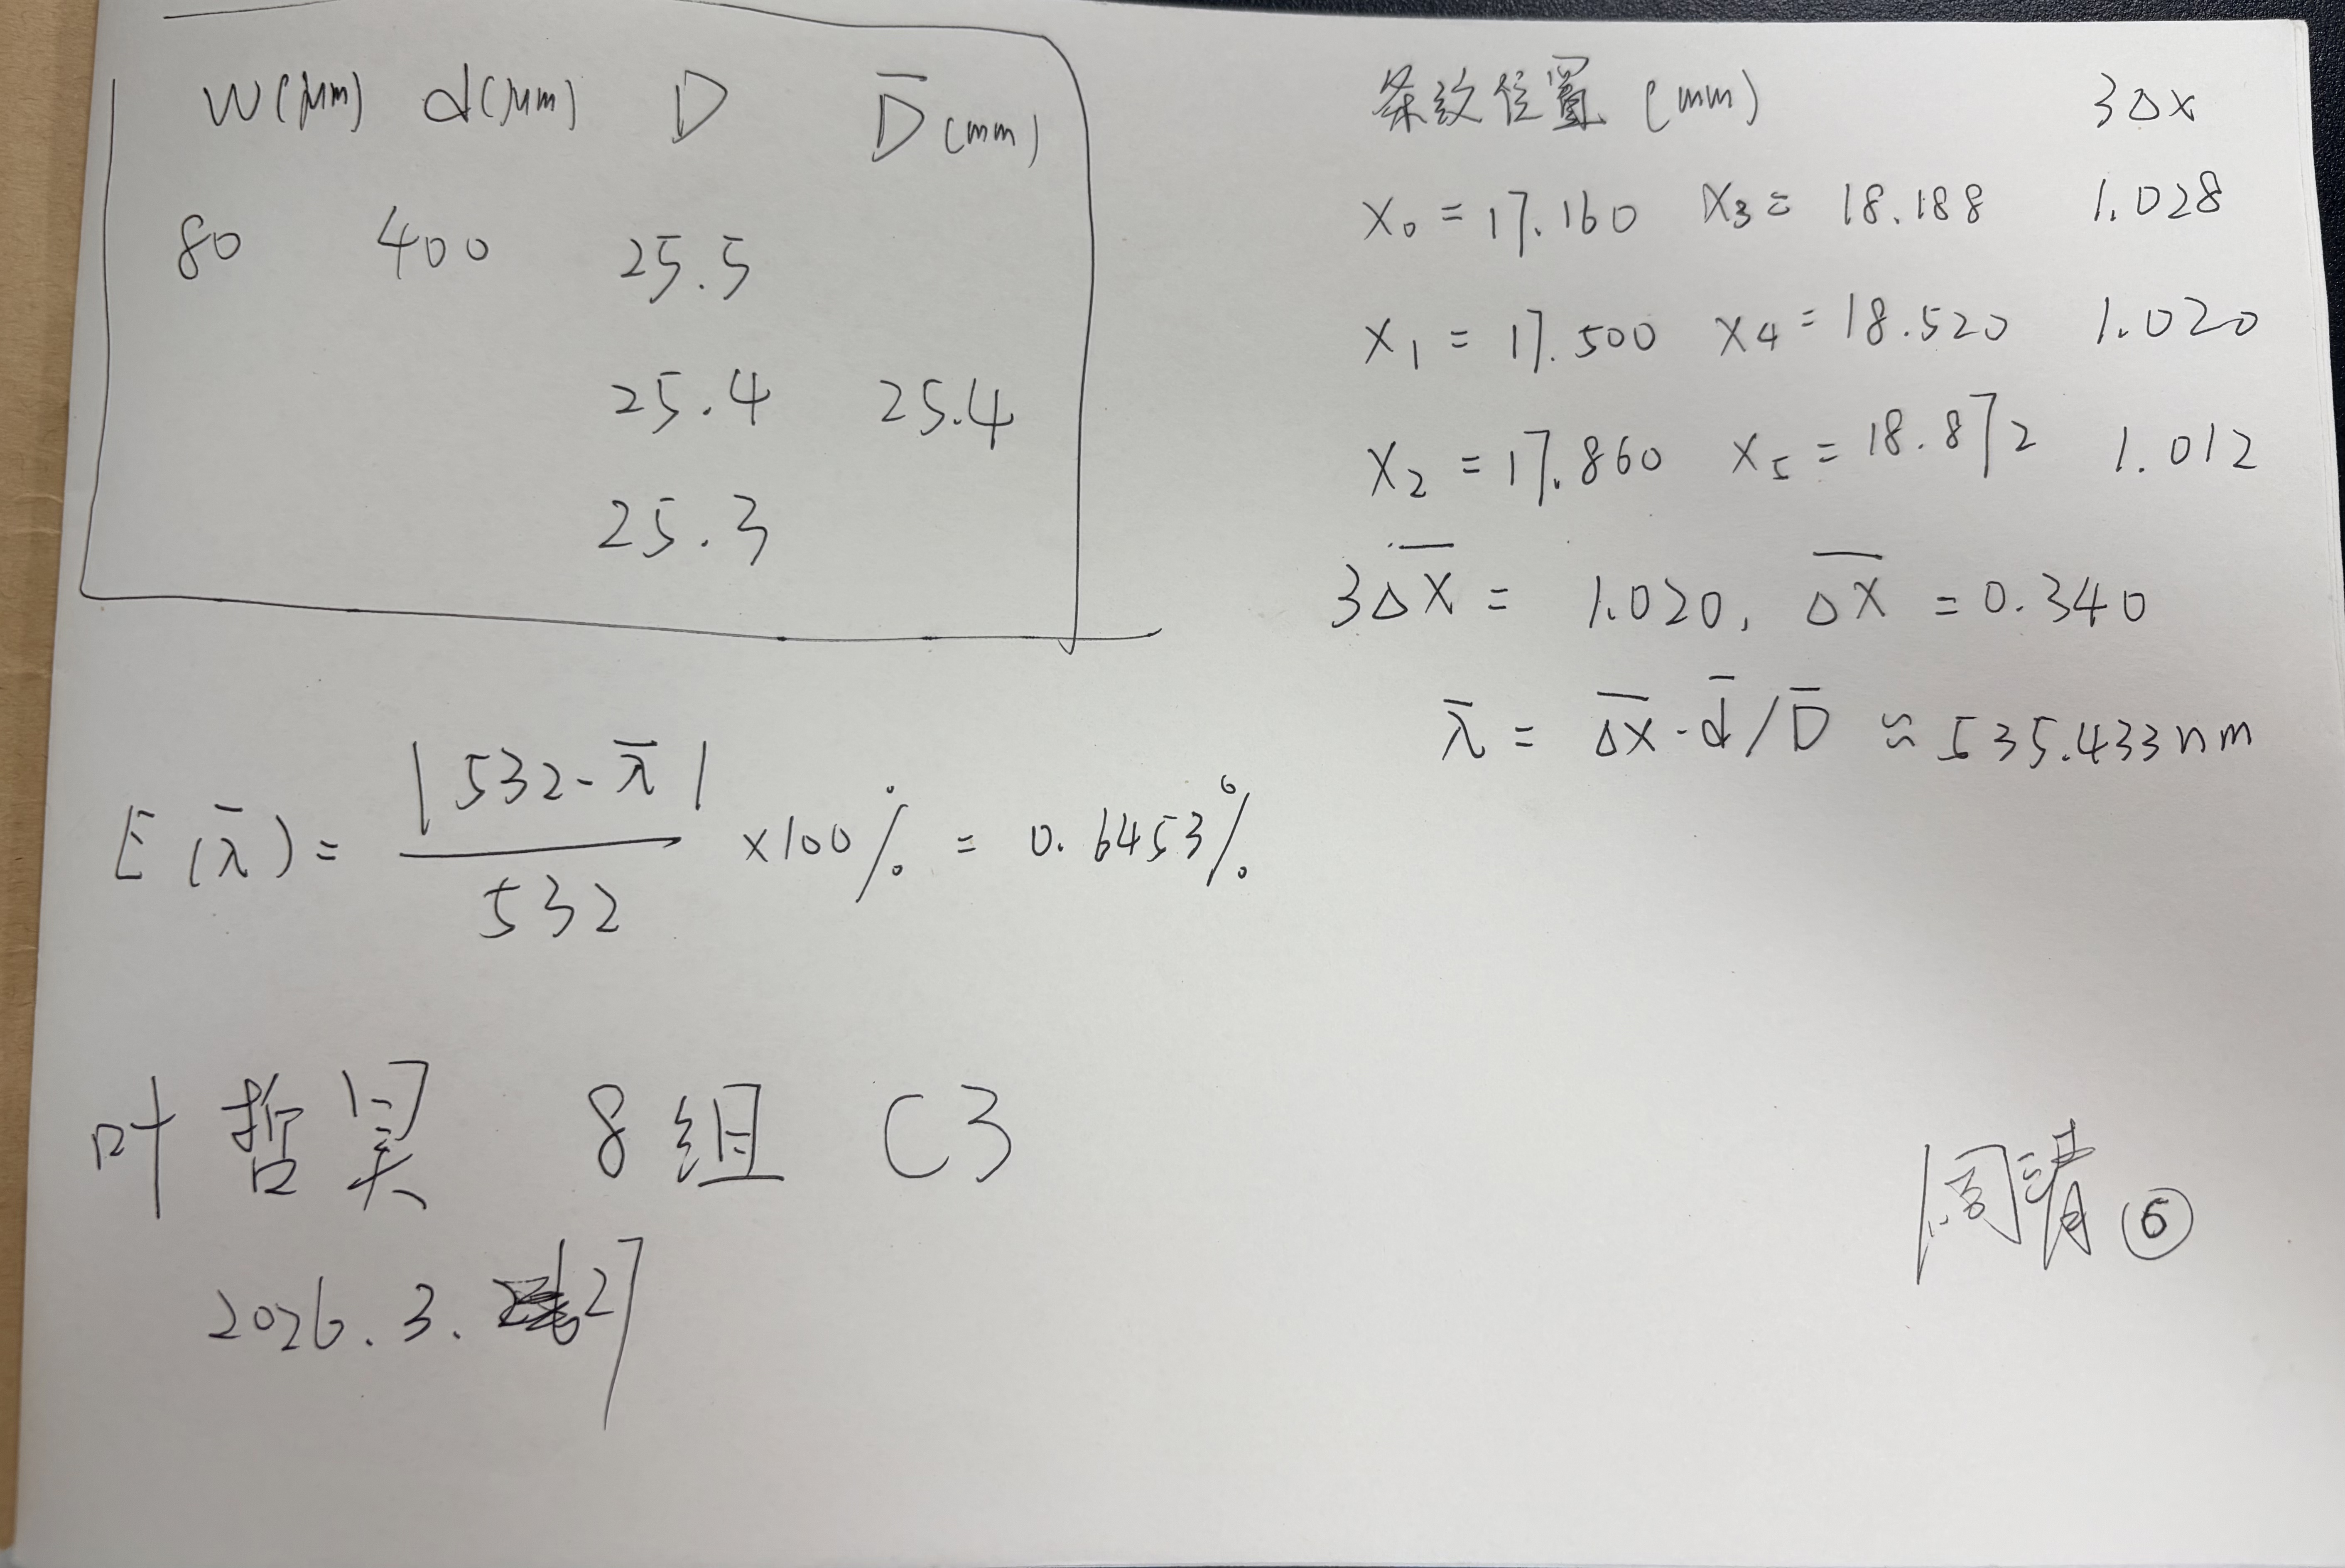
\includegraphics[width=0.9\textwidth]{实验数据（含签名）.jpg}
  \caption{杨氏双缝干涉实验原始数据记录（教师签字件）}
\end{figure}

\end{document}
